% =====================================================================
% Chapter 1 --- Introduction                                  [cross-cutting]
% Establishes the vision (UAM -> detect-and-avoid -> Sense -> the pipeline)
% and ties the three projects together as "one vision, three contributions".
% =====================================================================

Autonomous and remotely supervised aircraft are moving from isolated research
demonstrations toward routine operation in low-altitude urban airspace. For such
aircraft to fly safely among buildings, smaller drones, birds, and other
vehicles, they must build their own picture of the surrounding environment from
onboard sensors and react to it in real time. This dissertation addresses the
perception layer of that capability: detecting and tracking obstacles in three
dimensions from a moving aerial platform, using a multi-sensor fusion approach
that combines camera imagery and point-cloud data.

\section{Context: Urban Air Mobility and Situational Awareness}

Urban Air Mobility (UAM) refers to the emerging ecosystem of small, typically
electric vertical take-off and landing (eVTOL) aircraft intended for intracity
and intercity transportation of people and cargo \cite{straubinger2020uam}. A new
generation of vehicles, including those developed by Joby Aviation, Lilium, and
Embraer's subsidiary Eve Air Mobility, is being designed for this role, and with
them comes a regulatory and engineering push toward increasingly higher levels of
flight autonomy.

Operating in the urban canyon is fundamentally harder than operating at cruise
altitude. The airspace is cluttered and dynamic: static structures, moving
ground vehicles, other UAVs, and uncooperative air traffic share a small volume,
leaving little margin for error. A human pilot manages this through continuous
\emph{situational awareness}: perceiving nearby objects, estimating their
motion, and anticipating conflicts. An autonomous aircraft must reconstruct the
same awareness from its sensor suite. Building that awareness reliably, on
board, and in real time is the central enabling problem for safe autonomous
flight in cities (Figure~\ref{fig:uam_scene}).

\begin{figure}[H]
  \centering
  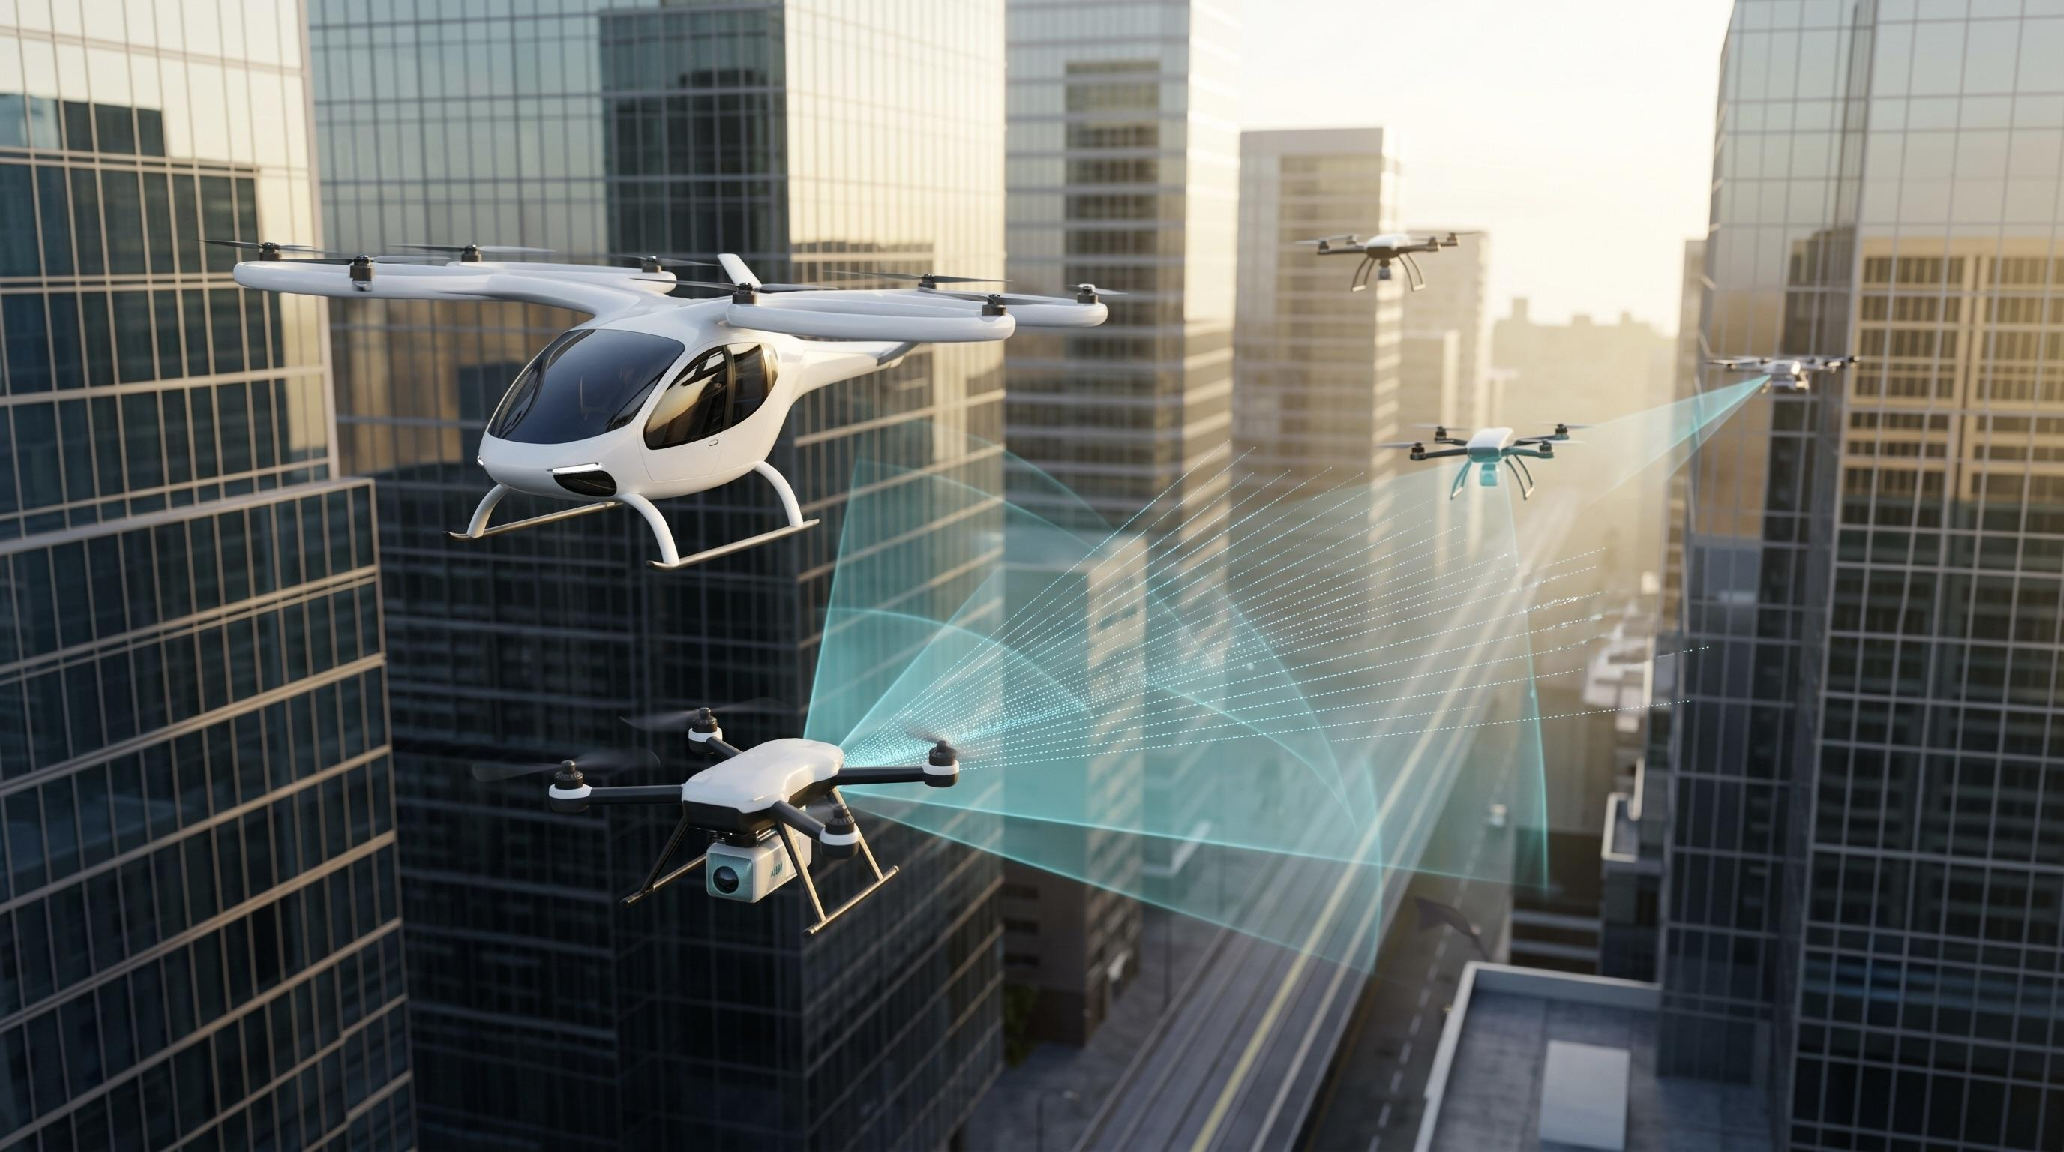
\includegraphics[width=\linewidth]{Cap1/uam_scene.pdf}
  \caption{Situational awareness for urban air mobility. An autonomous aerial
  vehicle sharing the urban canyon with other drones, manned eVTOL aircraft, and
  uncooperative traffic must perceive nearby obstacles from its onboard sensors
  (camera and point cloud) and react in real time --- the detect-and-avoid
  problem this dissertation addresses on its \emph{Sense} side.}
  \label{fig:uam_scene}
\end{figure}

This work was carried out within the FlyMov Engineering Research Center, a
partnership between the Aeronautics Institute of Technology (ITA), Embraer, and
the São Paulo Research Foundation (FAPESP), whose mission includes the
perception and decision-making technologies required for autonomous eVTOL
operation.

\subsection{Origin and Scope of the Three Studies}
\label{sec:origin}

This dissertation arose from three connected efforts that share one estimation
core and one guiding vision, yet differ in sensor, target, and setting. This
section describes how the three parts fit together.

The starting point, and the result-bearing core of the thesis, is the
range--bearing Extended Kalman Filter for tracking obstacles from a moving
platform (Chapter~\ref{cha:tracking}), developed and validated in simulation and
presented at the IEEE International Conference on Information Fusion (FUSION) in
2025 \cite{delima2025fusion}.

The second effort grew directly out of that publication. After the tracker was
presented at FUSION~2025, researchers from the UBADRON team of the Technische
Universit\"at Berlin (TU~Berlin), led by Prof.~Maarten Uijt de Haag, visited ITA.
Their team competes in the SPRIND ``Fully Autonomous Flight'' Challenge, in which
an autonomous UAV must operate without a Global Navigation Satellite System
(GNSS) and locate targets (people) on the terrain, a task with a clear
search-and-rescue motivation. They had a working
person-\emph{detection} front-end --- the early perception stage that turns raw
sensor data into per-object detections, before any tracking --- but lacked a
tracker, which is exactly what our FUSION work provided. The two groups therefore collaborated: TU~Berlin supplied
real flight data from their drones, and we adapted our estimator to their setting.
That setting is harder than the simulation: the only sensor is a single
monocular camera, so depth is unobservable and must be recovered from a
ground-plane assumption, and the platform pose is \emph{estimated} on board rather
than known, so its uncertainty must be propagated into the filter. The monocular
person tracker of Chapter~\ref{cha:monocular} is thus a distinct formulation,
linked to the FUSION tracker but adapted to a different sensor and a different
target; it was built during a three-month research stay at TU~Berlin.

The third effort addresses a different obstacle: the scarcity of annotated
three-dimensional aerial data needed to train the detection front-end of the
full camera--point-cloud pipeline. Chapter~\ref{cha:airsim} builds a synthetic
dataset in AirSim and trains and compares the detection networks on it.

The three studies are therefore distinct in their data and methods but unified by
the perception pipeline of Chapter~\ref{cha:pipeline}: \emph{one vision, three
contributions}.

\section{Detect-and-Avoid and the Sense Problem}

For any aircraft to share the airspace safely, it must be able to perceive
potential conflicts and act to prevent collisions. Aviation authorities codify
this requirement under the term \emph{Detect-and-Avoid} (D\&A), and it is a
mandatory element of the certification of autonomous and beyond-visual-line-of-sight
operations \cite{rtca2017do365}.
D\&A decomposes naturally into two coupled problems:

\begin{itemize}
  \item \textbf{Sense}, the \emph{perception} problem: detecting obstacles,
  estimating their three-dimensional position and extent, and tracking their
  motion over time from onboard sensors;
  \item \textbf{Avoid}, the \emph{decision and control} problem: planning and
  executing an evasive maneuver once a threat has been characterized.
\end{itemize}

This dissertation is concerned exclusively with the \textbf{Sense} side. The
avoidance problem (trajectory planning and control) is outside its scope and
is treated as a downstream consumer of the perception output. The essential
requirement that Sense places on Avoid goes beyond the obstacle's current
position. Avoid needs a \emph{calibrated} estimate of the obstacle's full state,
its position, velocity, and size, together with a trustworthy measure of the
uncertainty of that estimate, so that the avoidance logic can reason about
collision risk and time-to-conflict. Tracking where the obstacle \emph{is} is
therefore necessary but not sufficient. Because an evasive maneuver takes time to
plan and to fly, Avoid must reason about where the obstacle \emph{will be} several
steps ahead, and it is the perception layer that has to supply that forecast: a
track handed over without a prediction leaves the avoidance logic reacting to the
past. This is the main reason the perception output must include a temporal
tracking stage and not per-frame detections alone. The estimator developed here
supplies the forecast in the form that a recursive filter naturally affords:
its state carries position \emph{and} velocity together with a covariance, so
propagating the motion model forward yields a predicted position at any horizon,
accompanied by an uncertainty envelope that widens with that horizon. Richer
trajectory prediction, which would model the obstacle's intent rather than
extrapolate its kinematics, lies beyond the scope of this dissertation and is
taken up as future work in Chapter~\ref{cha:conclusions}. The size estimate, in
turn, bounds the spatial extent that the maneuver must clear. This emphasis on
calibrated uncertainty recurs throughout the thesis and motivates several of its
technical choices.

Within Sense, three perception sub-problems must be solved in sequence:
detection in two dimensions (locating objects in the image), detection in three
dimensions (lifting them into metric space), and tracking (maintaining their
state over time). The first two are powered by Convolutional Neural
Networks (CNNs); the third, the tracking stage, by recursive
Bayesian estimation.

\section{Problem Statement}

Concretely, we consider a UAV equipped with a camera and a source of
three-dimensional measurements (a LiDAR or a stereo/depth sensor) that must,
in real time and from a moving platform, (i) detect obstacles in its field of
view, (ii) estimate their three-dimensional position and size, and (iii) track
them over time, producing calibrated state estimates suitable for a downstream
avoidance module. Three characteristics make this difficult:

\begin{enumerate}
  \item \textbf{The observer is in motion.} Measurements are taken from a
  platform that is itself translating and rotating, so the obstacle's apparent
  motion in the sensor frame is not inertial and the sensor pose must be
  explicitly accounted for.
  \item \textbf{Sensing is noisy, and depth is hard to recover.} Every
  measurement carries noise in both range and bearing. Depth is the harder
  component: it is not \emph{directly} observable from a single monocular view,
  because the pre-image of a pixel is an entire ray, so it must be supplied either
  by an additional sensor or by an additional assumption about the scene. This is
  not to say that depth cannot be inferred from imagery at all. Modern learned
  monocular estimators do recover metric depth from a single image with useful
  accuracy \cite{bhat2023zoedepth,yang2024depthanything}, and the gap to an active
  range sensor has narrowed considerably; what remains true is that such an
  inference is indirect, and that its error is harder to characterize and to
  bound than that of a direct measurement, which matters for a certifiable
  estimator. This dissertation therefore recovers depth geometrically: from the
  point cloud where one is available (Chapters~\ref{cha:pipeline}
  and~\ref{cha:airsim}), and from a ground-plane constraint where the only sensor
  is a camera (Chapter~\ref{cha:monocular}). Even active range sensors degrade
  with distance, so the range noise is strongly range-dependent and must be modeled
  as such rather than assumed constant.
  \item \textbf{Aerial data are scarce and computational resources are limited.} Unlike ground
  autonomy, there is no abundance of annotated three-dimensional aerial
  datasets, and the perception stack must ultimately run on constrained onboard
  hardware.
\end{enumerate}

\section{Proposed Solution}
\label{sec:proposed_solution}

The approach taken here is a \emph{modular camera--point-cloud fusion pipeline},
modular in the sense that each stage exposes an explicit, low-dimensional
interface to the next and can therefore be trained, validated, and replaced
independently of the others. Figure~\ref{fig:pipeline_intro} shows the resulting
architecture end to end; it is the single artifact to which every chapter of this
dissertation contributes, and Chapter~\ref{cha:pipeline} develops it in detail.

A CNN detector first localizes objects in the image; each two-dimensional
detection is lifted into a viewing \emph{frustum} that bounds the corresponding
region of the point cloud; a point-cloud network estimates an amodal
three-dimensional bounding box (one that spans the object's full extent, including
the faces hidden from the sensor) within that frustum; and an Extended Kalman
Filter (EKF) tracks the resulting detections over time. This frustum-based
fusion follows the lineage of Frustum PointNets \cite{qi2018frustum}, adapted
here to the aerial sense-and-avoid setting.

\begin{figure}[H]
  \centering
  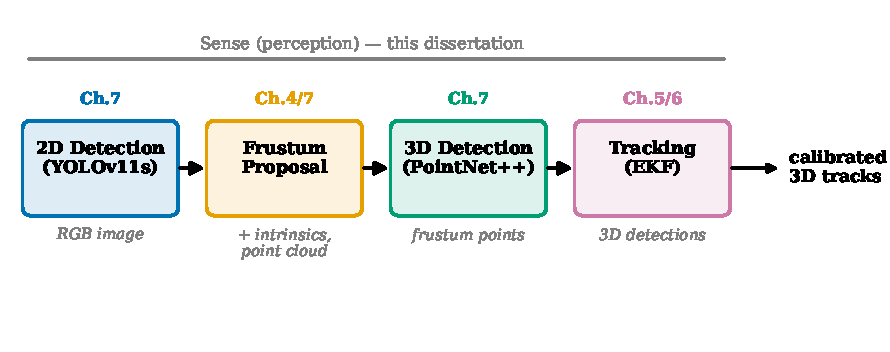
\includegraphics[width=\linewidth]{Cap4/pipeline_architecture.pdf}
  \caption{The proposed modular camera--point-cloud perception pipeline, shown
  here in overview. A 2D detector seeds a viewing frustum that crops the point
  cloud; a point-cloud network regresses a 3D box; and a recursive filter tracks
  the detections, outputting calibrated 3D tracks for the avoidance layer. Each
  of the three studies of this dissertation contributes one part of this single
  architecture, which Chapter~\ref{cha:pipeline} presents in full detail.}
  \label{fig:pipeline_intro}
\end{figure}

\subsection{Where the Point Clouds Come From}
\label{sec:cloud_provenance}

Because the pipeline consumes a point cloud at its second stage, it is worth
stating at the outset which sensor produces that cloud in each part of this work.
The three settings differ, and the distinction matters when reading the results.

\begin{itemize}
  \item In the pipeline as an \emph{architecture} (Chapter~\ref{cha:pipeline}),
  the cloud is whatever three-dimensional sensor the aircraft carries: a LiDAR, a
  stereo rig, or an RGB-D (depth) camera. The tracker consumes an abstract
  range--bearing measurement with a covariance and is indifferent to which of
  these produced it.
  \item In the simulated detection study (Chapter~\ref{cha:airsim}), the working
  cloud is produced by an \emph{idealized planar-depth camera} in AirSim, and not
  by a real LiDAR. A simulated $64$-beam LiDAR is available and is retained as an
  auxiliary channel, but at the altitudes of interest the targets are seen against
  the sky, where too few beams strike them to localize a target, whereas the dense
  depth image supplies the $10^{5}$--$3\times10^{5}$ points per frame that the
  point-cloud network needs. The idealization this entails, and its consequences
  for how the reported accuracy should be read, are stated explicitly in
  Section~\ref{sec:sensor_caveat}.
  \item In the real-flight study (Chapter~\ref{cha:monocular}) there is
  \emph{no} point cloud on the target at all. The only onboard sensor pointed at
  the person is a monocular camera, and the missing depth is recovered from a
  ground-plane constraint. A LiDAR appears in that study only offline, to survey
  the room and build the reference map against which the tracker is scored.
\end{itemize}

\section{Objectives}

The problem stated in Section~\ref{sec:proposed_solution} and the solution
sketched there translate into one overarching goal and three specific goals, one
per study. They are stated here in the order in which the dissertation pursues
them.

\subsection{General Objective}

To develop and validate the perception (\emph{Sense}) stack for UAV
detect-and-avoid in urban environments, designed as a structured modular
camera--point-cloud fusion pipeline whose tracking stage is
formulated, analyzed, and validated.

\subsection{Specific Objectives}

\begin{enumerate}
  \item To formulate the obstacle-tracking problem from a moving platform as a
  nonlinear Bayesian filtering problem, for which the EKF is the solution
  evaluated here, and to analyze
  rigorously the two natural choices of reference frame
  (global inertial versus local sensor), establishing their relationship and
  benchmarking the filter against the Cram\'er--Rao bound.
  \item To demonstrate the generality of the resulting framework by adapting it
  to monocular person tracking from a real UAV, explicitly propagating the
  camera-pose uncertainty into the estimator.
  \item To design the detection front-end of the pipeline, that is, the
  two- and three-dimensional detection stages that produce the measurements the
  tracker consumes, and to assemble a fully-annotated synthetic aerial dataset
  that enables its training in the absence of large-scale real data, and to
  evaluate the front-end, together with alternative detection paradigms, on a
  moving-observer campaign with three-dimensional detection and tracking metrics.
\end{enumerate}

\section{Contributions}

The dissertation makes the following contributions, organized as one overarching
system, the perception pipeline, and three self-contained studies that
realize and validate its components:

\begin{enumerate}
  \item \textbf{A rigorous treatment of EKF tracking from a moving platform}
  (Chapter~\ref{cha:tracking}). We give a unified derivation of the global- and
  local-frame formulations for spherical (range--bearing) measurements, prove
  that the two are \emph{mathematically equivalent} under a known platform pose
  and isotropic process noise, and characterize precisely the conditions under
  which they genuinely diverge. The formulation was presented at the IEEE
  International Conference on Information Fusion \cite{delima2025fusion}.
  \item \textbf{Generality of the framework, validated on real data}
  (Chapter~\ref{cha:monocular}). During a three-month research stay with the
  UBADRON team at the Technische Universit\"at Berlin (TU Berlin), the
  same estimator was extended to monocular person tracking from a UAV, where the
  platform pose is uncertain and depth is unobservable. A person detector trained on a union of
  complementary aerial datasets (spanning urban, rural near-range, and
  high-altitude regimes) supplies the image measurements; a ground-plane
  constraint recovers metric position from the single view; and the filter
  propagates the six-degree-of-freedom camera-pose covariance into its
  innovation, which an ablation shows to be necessary for statistical
  consistency under aggressive platform motion. The system is validated on real
  flights against a LiDAR-referenced ground truth.
  \item \textbf{A synthetic aerial dataset and detection front-end}
  (Chapter~\ref{cha:airsim}). A configurable, fully-annotated dataset built in
  AirSim addresses the scarcity of three-dimensional aerial data: a pixel-exact
  synthetic-composition scheme circumvents the simulator's unreliable annotation
  interfaces, and a geometric construction supplies trustworthy 3D boxes. The data
  are employed to train the CNN-based two- and three-dimensional detectors, which
  are then evaluated on a moving-observer campaign with the standard
  multi-object-tracking metrics of autonomous driving. The study further identifies
  foreground extraction, rather than the box regressor, as the dominant factor in 3D
  localization accuracy, and provides the first empirical comparison of the
  two-stage frustum design against the single-stage voxel paradigm on aerial data.
  \item \textbf{A systematic literature review} (Chapter~\ref{cha:relatedwork})
  following the PRISMA, Kitchenham, and Wohlin methodologies, which establishes
  that frustum-based camera--point-cloud detection has not previously been
  brought to UAV sense-and-avoid, and locates this work within that gap.
\end{enumerate}

\section{Publications}

The tracking formulation of Chapter~\ref{cha:tracking} was published as:
de~Lima, Dias, and Maximo, \emph{Extended Kalman Filter-Based Object Tracking
Using Global and Local Frames}, IEEE International Conference on Information
Fusion (FUSION), 2025 \cite{delima2025fusion}. The real-data study of
Chapter~\ref{cha:monocular}, developed with the UBADRON team of the Chair of
Flight Guidance and Air Transport at TU~Berlin, is in preparation for publication.

\section{Outline of the Dissertation}

The remainder of the dissertation is organized so that a shared foundation
supports three self-contained studies. Chapter~\ref{cha:background} establishes
the common theoretical framework, comprising recursive Bayesian estimation and the
EKF, coordinate frames, motion and measurement models, consistency metrics, and the
neural-network building blocks from which every later chapter draws.
Chapter~\ref{cha:relatedwork} reviews the literature and substantiates the
research gap. Chapter~\ref{cha:pipeline} presents the perception pipeline as a
single architecture and shows how the three studies map onto it. The three study
chapters then follow, each self-contained with its own methodology and results:
Chapter~\ref{cha:tracking} develops and analyzes the EKF tracker in global and
local frames; Chapter~\ref{cha:monocular} extends it to monocular tracking from a
real UAV; and Chapter~\ref{cha:airsim} builds the synthetic dataset and the
detection front-end. Chapter~\ref{cha:conclusions} synthesizes the three studies,
revisits the contributions, and outlines future work toward an integrated,
onboard sense-and-avoid system.

\section{Note on the Use of Artificial-Intelligence Tools}
\label{sec:ai_disclaimer}

In the interest of transparency, the author discloses the use of
Artificial-Intelligence (AI) assistants during the preparation of this
dissertation. AI-based tools (large language models) were used as a writing aid,
to improve the clarity, grammar, and flow of the English text, to help structure
and format \LaTeX{} and to assist with routine plotting and figure-generation
code. They were \emph{not} used to produce experimental results: every model,
derivation, experiment, dataset, and numerical result reported here was designed,
implemented, executed, and verified by the author. All technical claims were
checked against the underlying data and code, and the author takes full
responsibility for the content.
